\documentclass[conference]{IEEEtran}
\IEEEoverridecommandlockouts
% The preceding line is only needed to identify funding in the first footnote. If that is unneeded, please comment it out.
\usepackage{cite}
\usepackage{amsmath,amssymb,amsfonts}
\usepackage{algorithmic}
\usepackage{graphicx}
\usepackage{textcomp}
\usepackage{xcolor}
\interdisplaylinepenalty=2500
\def\BibTeX{{\rm B\kern-.05em{\sc i\kern-.025em b}\kern-.08em
    T\kern-.1667em\lower.7ex\hbox{E}\kern-.125emX}}
\begin{document}

\title{Enhancing Robust Node Classification via Information Competition: an improved adversarial resilience method for graph attacks
\\
% {\footnotesize Improving Adversarial Resilience for Graph Attacks}

% \thanks{Identify applicable funding agency here. If none, delete this.}
}

\author{\IEEEauthorblockN{1\textsuperscript{st}Yong Huang}
\IEEEauthorblockA{\textit{Zhejiang Laboratory} \\
Hangzhou, China \\
yhuang@zhejianglab.com}
\and
\IEEEauthorblockN{2\textsuperscript{nd} Qiao Han}
\IEEEauthorblockA{\textit{Zhejiang Laboratory} \\
Hangzhou, China \\
hanq@zhejianglab.com}
\and
\IEEEauthorblockN{3\textsuperscript{rd} Xinling Guo}
\IEEEauthorblockA{\textit{Zhejiang Laboratory} \\
Hangzhou, China \\
guoxl@zhejianglab.com}
\and
\IEEEauthorblockN{4\textsuperscript{th} Yiteng Zhai}
\IEEEauthorblockA{\textit{Zhejiang Laboratory} \\
Hangzhou, China\\
ito@zhejianglab.com}
\and
\IEEEauthorblockN{5\textsuperscript{th} Yao Yang}
\IEEEauthorblockA{\textit{Zhejiang Laboratory} \\
Hangzhou, China\\
yangyao@zhejianglab.com}
% \and
% \IEEEauthorblockN{6\textsuperscript{th} Given Name Surname}
% \IEEEauthorblockA{\textit{dept. name of organization (of Aff.)} \\
% \textit{name of organization (of Aff.)}\\
% City, Country \\ 
% email address or ORCID}
}

\maketitle

\begin{abstract}
Graph neural networks (GNNs) have demonstrated their effectiveness in facilitating node classification and a range of graph-based tasks. However, recent studies have revealed that GNNs can be vulnerable to adversarial attacks, posing challenges for real-world applications. 
Despite various defense strategies, ranging from attack-agnostic defence to attack-oriented defence, have been proposed to mitigate the impact of adversarial attacks on graph data, effectively learning robust graph representation remains a challenge. 
This paper introduces a novel information Competition-based Framework for Graph Neural Networks (i.e., \textit{iC}-GNN framework, e.g., \textit{iC}-GCN, \textit{iC}-GAT, etc.) to enhance the robustness of GNNs against adversarial attacks in node classifications. Through the use of graph reconstruction and low-rank approximation, our approach learns diversified graph representations to collaboratively accomplish node classifications. Meanwhile we utilize mutual information constraints on different graph representations to ensure diversity on features.
The results of experiments indicate that, under the proposed framework, Graph Convolutional Network (\textit{iC}-GCN) can surpass other graph defense frameworks in defending against various target/non-target adversarial attacks under both evasion and poisoning training settings. Additionally, we have extended this idea to GraphSage (\textit{iC}-SAGE) and Graph Attention Network (\textit{iC}-GAT) models, all three models can effectively defend, demonstrating similar robustness against adversarial attacks. This indicates the strong scalability of our framework, holding promise for a variety of graph learning tasks.
\end{abstract}

\begin{IEEEkeywords}
Graph Neural Networks, Adversarial Attacks, Adversarial Defences, Robust Graph Neural Networks, Mutual Information Estimation, Information Competition
\end{IEEEkeywords}

\section{Introduction}

The invention of Graph Neural Networks (GNNs)  \cite{Defferrard2016ConvolutionalNN} \cite{velickovic2018graph} \cite{Wu2019ACS} \cite{Sun2019InfoGraphUA} marks a revolutionary shift in the understanding of graph data, from structured feature engineering to representation learning \cite{Chen2019GraphRL} \cite{Khoshraftar2022ASO}. It have demonstrated remarkable capabilities and ubiquitous applications across various domains, including artificial intelligence for science \cite{Li2022MultiphysicalGN}, recommendation and search system \cite{Yang2021ConsisRecEG} \cite{Wang2022GNNbasedRA}, knowledge graph reasoning\cite{Qiu2023LogicalEO}, and analysis of social networks\cite{Si2022RecGNNRO}. However, recent studies \cite{xu2019topology} \cite{Zgner2019AdversarialAO} have shown that deep neural network models are vulnerable to adversarial attacks, and GNNs are even more fragile because attackers can exploit the unique relationship information (the edges) \cite{Zgner2018AdversarialAO}. A carefully calculated disturbance on original test data, even if very slight and imperceptible, can easily lead these models to wrong outputs. Such negative results significantly hinder the applicability of these models, posing challenges for these real-world applications.


Defence mechanisms for GNNs can be classified into attack-agnostic defences and attack-oriented defences. Attack-agnostic defence exposes the model to adversarial examples during training to improve the robustness of their models against adversarial attacks. Attack-oriented defence is another effective way of defense is to detect and remove attacks, under the assumption that data have already been polluted. 
The intrinsic idea of attack-agnostic defences and attack-oriented defences is to perform information pruning (i.e., node/edges features or hidden representation layers) on graph data. However, existing approach mostly focus on the introduction or improvement of single pruning techniques, lacking the organic integration of multiple pruning methods and the extraction of diverse features from the original data. This limitation restricts the upper limit of model accuracy and robustness.

To address this problem, we propose a graph information competition framework for Graph neural networks, a novel model that fortifies GNNs against adversarial attacks on node classifications. Our approach uses graph reconstruction and low-rank approximation to learn diversified graph representations and promotes competition and collaboration among different graph representation parts.
In the competition stage, we apply mutual information constraints to different representation methods, allowing them to independently complete tasks while extracting information that is as different as possible. In the collaboration stage, multiple perspectives are adopted to learn from different pruning results. We believe that this information constraint can yield both effective (discriminative ability) and meaningful (decoupling ability) features, thereby enhancing the model's robustness (removing ineffective/adversarial features) while ensuring its accuracy.


The core innovations and contributions of this paper are:
\begin{itemize}
    \item We propose \textit{iC-}GNN (including \textit{iC-}GCN, \textit{iC-}SAGE and \textit{iC-}GAT) methods that incorporates various defense methods into information competition process to jointly enhance adversarial robustness, providing new insights on leveraging graph model ensemble diversity for defense.
    \item Our approach leverages graph reconstruction and low-rank approximation to acquire diverse graph representations for collaborative fulfillment of node classification tasks. Meanwhile we utilize mutual information constraints on different graph representations to ensure feature diversity.
    \item Through extensive experiments on three public graph datasets, we demonstrate information Competition-based Graph Convolutional Network Framework (\textit{iC-}GCN) significantly outperforms state-of-the-art defense methods against diverse trarget/non-target adversarial attacks under both evasion and poisoning training settings. Our approach exhibits consistent superiority in defending against various attack types and magnitudes.  
\end{itemize}

The remainder of this paper is organized as follows: Section 2 reviews related prior works. Section 3 elaborates on the principles and details of the proposed method GNN-ICP. In Section 4, we detail experimental setup and results. Finally, Section 5 concludes the paper.



\section{Related Work}

Our work builds upon three categories of recent research: graph neural network, graph adversarial attacks, and robust graph neural networks, encompassing a comprehensive exploration of the evolving landscape in graph-based representation learning and adversarial attacks/defences.

\subsection{Graph Neural Networks}
%We provide a brief overview of representative Graph Neural Networks, 

Graph Neural Networks (GNNs)\cite{Zhou2018GraphNN} strive to acquire and generalize significant representations of graph data. These networks typically employ message passing to capture intricate relationships and dependencies within graph data structures, aggregating messages between nodes through the edges. By leveraging connectivity patterns, GNNs update and enhance node representations based on the features and connections of neighboring nodes, facilitating diverse downstream tasks such as node classification, link prediction, and graph-level classification.


The Graph Convolutional Network (GCN) \cite{kipf2017semi} is a type of Graph Neural Network (GNN) designed to perform learning tasks on graph-structured data. At the core of GCNs is the graph convolutional layer, which enables the propagation of information across the graph while considering the graph's topology, each node aggregates and combines information from its neighboring nodes. This process allows GCNs to learn expressive node representations by capturing the local graph structure.
Another variant, the Graph Attention Network (GAT) \cite{velickovic2018graph}, integrates attention mechanisms to selectively aggregate information from different neighbors, assigning greater importance to relevant nodes for the target task, allowing it to focus more on relevant nodes for a given task. 
GraphSage \cite{hamilton2017inductive} is an inductive framework that performs neighborhood sampling and aggregation, allowing it to scale to massive graphs while still capturing important structural information. During the sampling stage, for each node it samples a fixed number of neighbors or a fixed-size subgraph. In the aggregation stage, each node aggregates information from its sampled neighbors through a learnable aggregation function such as mean, max, or attention mechanism.

Other variant like Graph U-Net model \cite{gao2019graph}, R-GCNs \cite{Schlichtkrull2017ModelingRD}, Deep Graph Infomax model \cite{velickovic2018deep} are also popular in various graph tasks. For example, R-GCNs \cite{Schlichtkrull2017ModelingRD} models relational knowledge graph data with Graph Convolutional Networks, LinKG \cite{Zhang2019OAGTL} links large-scale heterogeneous entity graphs.

 \begin{figure}
  \centering
  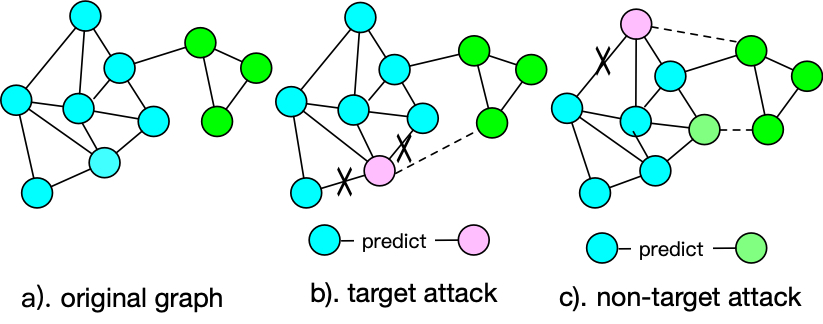
\includegraphics[width=.5\textwidth]{attack.jpg} %1.png是图片文件的相对路径
  \caption{the visualization of targeted/non-target Attack, a dashed line indicates a fabricated edge connection, a cross sign denotes the deletion of edges.} %caption是图片的标题
  \label{attack} %此处的label相当于一个图片的专属标志,目的是方便上下文的引用
\end{figure}

\subsection{Graph Adversarial Attacks}

Since most graph neural networks aggregate and combine information from its neighboring nodes, graph adversarial attacks are trying to perturb graph structures or node features to influence GNN models while remaining unnoticeable to users. These adversarial attack methods can be divided into following categories:

\subsubsection{Targeted/Non-target Attack}. The objective of targeted attacks \cite{Zgner2018AdversarialAO} is to alter the prediction of a particular target node within a graph. These targeted attack methods can be classified into two types: direct attacks, which manipulate the target node directly, and influencer attacks, which indirectly manipulate the target node by altering other nodes. Non-targeted attacks \cite{Zgner2019AdversarialAO} aim to reduce the overall model performance and influence. the goal of non-target attack is to increase the misclassification rate of a node classification algorithm achieved after training on the graph data.

Targeted and non-target Attack are visually represented in figure \ref{attack} from left to right, figure a) presents original graph visualization, figure b) presents target attacks which trying to misclassify certain target nodes by removing or adding edges like the pink node, figure c) presents non-target attack which aim to influence the task of classifying all graph nodes. 

\subsubsection{Poisoning/Evasion Attack} Poisoning attacks \cite{li2020deeprobust} try to attack the model by changing graph data during training phase, the attacker modifies the training data by adding or altering a subset of nodes or edges in the graph, misleads the GNN model during the training phase. Evasion attacks \cite{li2020deeprobust} perturb graph data for a trained model during test phase, the attacker carefully crafts perturbations or modifications to the graph structure or node features, intending to cause the GNN to misclassify the target nodes or predict incorrect outcomes.


\subsection{Graph Adversarial Defences}

Defence mechanisms for GNNs categories following this survey \cite{sun2022adversarial} can be classified into \textbf{Attack-agnostic Defence} and \textbf{Attack-oriented Defence}.
Attack-agnostic defence exposes the model to adversarial examples during training to improve the robustness of their models against adversarial attacks. typical methods include GIB \cite{Tishby2000TheIB}, RGCN\cite{Zhu2019RobustGC}. Attack-oriented defence is another effective way of defense to detect and remove attacks, under the assumption that data have already been polluted. typical methods includes GCNSVD \cite{Entezari2020AllYN}, GCN-LFR\cite{chang2021not}.

GCNSVD\cite{Entezari2020AllYN} firstly argues the weakness of Nettack and leveraged SVD to defend against Nettack. GCN-LFR \cite{chang2021not} further proves that the low frequency components of the symmetric normalized Laplacian, which is usually used as the convolutional filter in GCNs could be more robust against structural perturbations but not all low-frequency components are robust to adversarial attacks. \cite{Bojchevski2019CertifiableRT} considers graph structural perturbation while \cite{Zgner2019CertifiableRA} designs robustness certificates to measure the safety of individual nodes and considered attribute perturbation. 

Another concept of robust GNNs is Information Bottleneck \cite{Tishby2000TheIB} which originally emerged in information theory that explores the trade-off between compression and relevance in data representation, it aims to find a balance between maintaining relevant information in the input data and discarding unnecessary details. The graph information bottleneck (GIB) \cite{wu2020graph}  is an Information Bottleneck framework applied to graph-structured data, GIB tries to capture the essential structure information in the graph while eliminating redundant graph information to balance expressiveness and robustness of learned representation.


\subsection{Summary}
In this section, we start by presenting an introduction to graph neural networks. Then, we establish the attack threat model for GNNs by considering perturbations in the graph. Finally we discuss common knowledge about graph defense models. As far as our knowledge extends, there has been no prior study on improving the robustness of graph representation through information competition.

\begin{figure*}
  \centering
  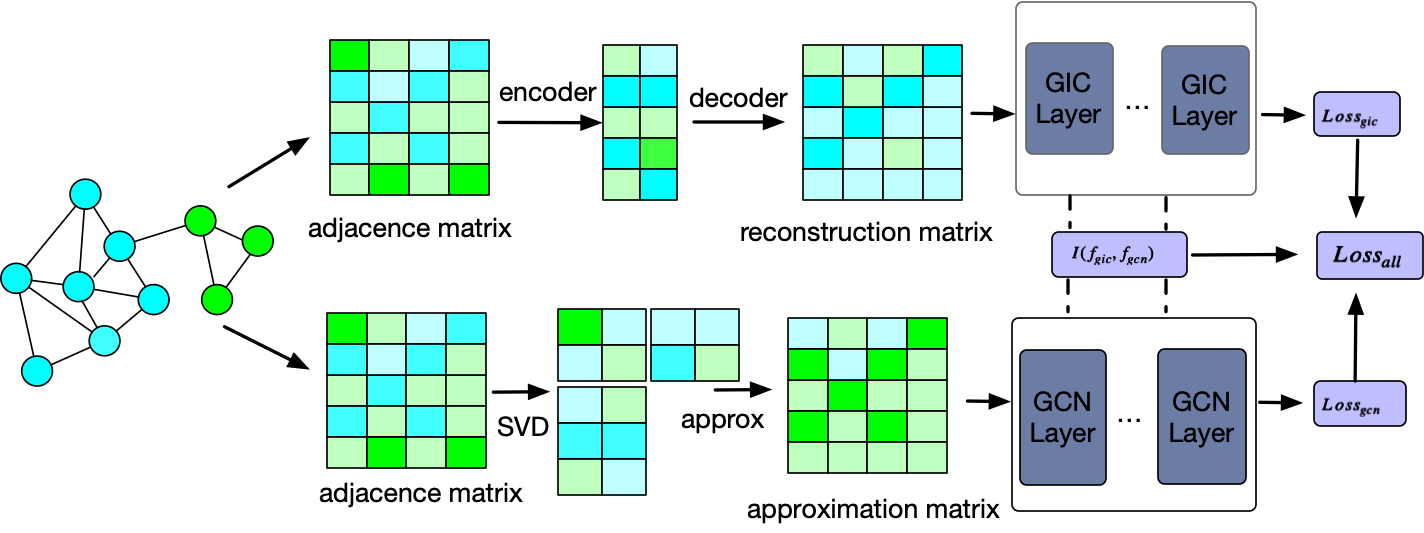
\includegraphics[width=.9\textwidth]{frame1.jpg} %1.png是图片文件的相对路径
  \caption{The overall framework of Graph Information Competition, we leverage different representation parts compete and collaborate with each other to acquire a comprehensive graph representation, so that we can enhance the robustness of our graph neural network model in node classification tasks} %caption是图片的标题
  \label{frame} %此处的label相当于一个图片的专属标志,目的是方便上下文的引用
\end{figure*}

\section{Proposed Methods}

Based on aforementioned exploration, to enhance the robustness against adversarial attacks, we introduce a novel framework using the idea of \textbf{information Competition for Graph Neural Networks} (i.e., \textit{iC-}\{Graph Method\}, e.g., \textit{iC-}GNN, \textit{iC-}GAT, etc.). We begin by outlining the overarching defensive framework before delving into the intricate specifics of the technical details, including several key components such as graph convolutional layers, information competition, mutual information estimation, and loss function.

\subsection{An Information Competition Framework}

We introduce a graph information competition framework, as illustrated in figure \ref{frame}. Our approach incorporates two novel modifications compared to existing methods: (1)Our approach leverages graph reconstruction and low-rank approximation to acquire diverse graph representations for collaborative fulfillment of node classification tasks. (2) we utilize mutual information constraints on different graph representations to ensure feature diversity for defending against attacks. 

the rest of this section introduces graph reconstruction and low-rank approximation, and how to diversify graph representations, foster competition and collaboration among different graph representation components, ultimately leading to improved node classification accuracy across diverse attack scenarios. Table \ref{lookup-table} summarized the most frequently used notations in this paper.



\begin{table}
    \centering
    \caption{A lookup table of frequently used notations}
    \begin{tabular}{c|l}
    \hline
    Notation & Description \\
    \hline
     $G$  & original graph\\
     \hline
     $v_i$  & node $i$ in $G$ \\
     \hline
     $G^{v_i}$ & graph component containing $v_i$ \\
     \hline
     $N(v_i)$ & a set of neighbors of node $v_i$\\
     \hline
       $A$  & adjacency matrix originating from $G$ \\
    \hline
     $A'$ & adjacency matrix originating from $A$\\
     \hline
     $X$  & node feature matrix  \\
    \hline
    $X'$ & feature matrix originating from $A$\\
     \hline
     $\sigma$  & the activation function  \\
    \hline
     $W$  & the weight matrix  \\
    \hline
    \end{tabular}
    \label{lookup-table}
\end{table}


\subsection{diversity of Graph Representation}

The key idea of graph information competition driven from Information Competing Process \cite{hu2019information} in which different representation parts compete and collaborate with each other to diversify the information. Given 2 diversified representation parts $[x,y]$ in node classification task, the objective is to promote diversity in the representations while avoiding domination of any part during node classification tasks. To achieve this, we aim to minimize the mutual information between $x$ and $y$. Furthermore, we utilize the representations of both $x$ and $y$ to maximize the mutual information between $x$ (or $y$) and $z$, where $z$ is the target of node classification task.

Our diversified graph representation is constructed by combining two essential components: low-rank approximation and graph encoder. The first part, low-rank approximation, aims to capture and represent the fundamental structure and patterns of the graph in a more compact form. the second component is responsible for encoding the graph's nodes and edges into a meaningful and expressive latent space. Both of them are representative graph representation methods, and they ensure a comprehensive and informative encoding of the graph's structure and characteristics.

\subsubsection{Low-rank approximation} Low-rank approximation serves as a popular approach for mitigating high-rank attacks when utilizing a lower-rank approximation of the graph structure. In this context, by considering the adjacency matrix A and the feature matrix X, low-rank approximation leverages Singular Value Decomposition (SVD) \cite{Wall2002SingularVD} or SVD-related methods to decompose the graph's adjacency matrix into a summation of rank-r matrices. The SVD of the adjacency matrix $A$ can be calculated as follows:
\begin{equation}
\label{svd-form1}
 A= U \Sigma V^T
\end{equation}
where U is an orthogonal matrix containing the left singular vectors,
$\Sigma$ is a diagonal matrix containing the singular values, $ V^T $ is the transpose of an orthogonal matrix containing the right singular vectors. Then the rank-r approximation of adjacency matrix $A'$ is computed as follows:
\begin{equation}
\label{svd-form2}
A' \approx U_r \Sigma_r V_r^T = \sum_{i=1}^r u_i \sigma_i v_i ^T
\end{equation}

where $U_r$ and $V_r$ are the matrices containing the top-r singular vectors and $\Sigma_r$ is the diagonal matrix containing only the r singular values.

\subsubsection{Graph Reconstruction} Graph reconstruction \cite{Kipf2016VariationalGA} \cite{Winter2021PermutationInvariantVA} is another graph representation method using encoder-decoder to generate non-uniform random numbers by transforming some base distribution.
Given an adjacency matrix $A$ and a node feature matrix $X$, the encoder first generates the latent representation $Z$ for each node in the graph:
\begin{equation}
\label{graph-encoder-form1}
Z = f_{\text{encoder}}(A, X)
\end{equation}
where $f_{\text{encoder}}$ represents the encoding function that maps the input graph structure and node features to the latent space.
The decoder then reconstructs the adjacency matrix and the node feature matrix from the latent representations:
\begin{equation}
\label{graph-encoder-form2}
A' = g_{\text{decoder}}(Z), \quad X' = h_{\text{decoder}}(Z)
\end{equation}
where $g_{\text{decoder}}$ and $h_{\text{decoder}}$ represent the decoding functions for the adjacency matrix and node features.

\subsection{Graph Information Competition}

In this section, we will explore Graph Convolutional Layers (GCN Layer or GCNLayer) and Graph Information Competition layers (GIC Layer or GICLayer). Both the representations of GCNLayer and GICLayer are bound by mutual information constraints which we will discuss in next subsection.

\subsubsection{GCN Layer} 
\label{section:gcnlayers}
Though a number of different GCN-based methods have been proposed, in this part, we mainly focus on a representative GCN model \cite{kipf2017semi}.For a node $v_i$, given the adjacency matrix $A$, the feature matrix $X$, its representation after aggregation of its neighbors' embeddings can be computed as:
\begin{equation}
\label{gcn-form1}
H^{(l+1)} (v_i)= \sigma(\tilde{A}H^{(l)}(v_i)W^{(l)}) 
\end{equation}
where $H^{l+1}(v_i)$ is the node representation matrix at layer $l+1$ of node $v_i$, or or in the equivalent form $H^{(l+1)}(v_i)$ is defined as:
\begin{equation}
\label{gcn-form2}
H^{(l+1)}(v_i) = \sigma(\hat{D}^{-\frac{1}{2}}\hat{A}\hat{D}^{-\frac{1}{2}}H^{(l)}(v_i)W^{(l)})
\end{equation}


where $\hat{A}$ represents the symmetrically normalized adjacency matrix $(A + I)$, $\hat{D}$ is the diagonal matrix containing the degree information of $\mathbf{A}$ with $\tilde{d}_{ii} = \sum_j \tilde{A}{ij}$, and $W^{(l)}$ is a learnable weight matrix, $\sigma$ is a
non-linear activation function such as ReLU or sigmoid. Then we get graph convolutional layers output $f(v_i)$ as follows:
\begin{equation}
\label{gcn-form3}
f(v_i) = \sigma (\hat{D}^{-\frac{1}{2}}\hat{A}\hat{D}^{-\frac{1}{2}}H_v^{(L)}(v_i)W^{(L)})
\end{equation}
where $L$ is the total number of layers, $H^{(L)}(v_i)$ represents the node $i$ representation matrix at the final layer.

\subsubsection{GIC Layer} 
our GIC Layer formally adopts graph encoder \cite{Kipf2016VariationalGA}  as the hidden representations of nodes in each convolutional layer. Denote $h^{(l)}(v_i)$ as the latent representation of node $v_i$ in layer $l$, we define graph encoder based graph convolution as follows:
\begin{equation}
\label{gic-form1}
h^{(l+1)}(v_i) &= \sigma (z(l)z(l)^t)
\end{equation}
where $z(l)$ is an graph encoder written as follows:
\begin{equation}
\label{gic-form2}
q(z(l)|h^{(l)}(v_i),A)=N(\mu_i^{(l)},diag(\sigma_i^{(l)}))
\end{equation}
where $\mu_i^{(l)}=GCNLayer(h^{(l)}(v_i),A)$ is the the matrix of mean vectors , similarly $diag(\sigma_i^{(l)})=GCNLayer(h^{(l)}(v_i),A)}$. here $\sigma(*)$ is the logistic sigmoid or ReLU activation function, and the GCNLayer is introduced in section \ref{section:gcnlayers}.




\subsubsection{GCN-based Layers} While we discuss the prominent GCN Layers, we also present a concise mathematical representation of GraphSage Layers and GAT Layers as alternatives to GCN Layers. The formula for the GraphSage Layer is given below:
\begin{equation}
\label{GCN-based-form1}
 h^{(l+1)}(v_i) = \sigma \left(W^{(l)} \cdot \text{CONCAT}(h^{(l)}(v_i), h_{\mathcal{N}(v_i)}^{(l)})(v_i) \right) 
 \end{equation}

where $h_{\mathcal{N}(v_i)}^{(l)}(v_i)$ is an mean-basd or LSTM-based aggregator,  $\mathcal{N}(v_i)$ is the set of neighbors of node $v_i$, and $ h_{\mathcal{N}(v)}^{(l)}$ is the aggregated embeddings of the neighbors of $v_i$ at layer $(l)$, $W$ is the learnable weight matrix. the GAT layer is written as follows:
\begin{equation}
\label{GCN-based-form2}
  h^{(l+1)}(v_i) = \sigma \left( \sum_{j \in N_i} \alpha_{ij}^{(l)} W^{(l)} h_j^{(l)}(v_i) \right) 
\end{equation}

where $h_v^{(l)}$ is the representation of $v_i$ at layer $l$, $N_i$ represents the set of neighboring nodes of node $v_i$, $\alpha_{ij}^{(l)}$ is the attention coefficient for the connection between nodes $i$ and $j$ at layer $l$, and $\sigma$ is the activation function.



\subsection{Mutual Information Estimation}

Mutual information is a measure of the amount of information shared between two random variables, it quantifies the extent to which the knowledge of one variable reduces uncertainty about the other.
We define this mutual information $I(f_{gic},f_{gcn})$ as the representations of GICLayer and GCNLayer, to simplify this we use $I(x,y)$ to replace $I(f_{gic},f_{gcn})$, written as follows:

%\setlength{\arraycolsep}{0.0em}
\label{eqn_example}
\begin{eqnarray}
\begin{split}
I(x,y) &= \sum_{x \in X} \sum_{y\in Y}p(x,y)log_2 \frac{p(x,y)}{p(x)p(y)} \\
 & = E_{p(x,y)} log_2 \frac{p(y|x)}{p(y)} \\
& = KL[p(y|x)p(x)||p(x)p(y)]
\end{split}
\end{eqnarray}
%\setlength{\arraycolsep}{5pt}
where $KL(*)$ is KL-divergence, $I(x,y)$ is the the KL-divergence between $p(x,y)$ and $p(x)p(y)$, and we use $r(y)$ to perform variational estimation of $p(y)$, from $KL(p(y),r(y)) \ge 0$ we can infer:
%\setlength{\arraycolsep}{0.0em}
\begin{eqnarray}
\label{eqn_example}
\begin{split}
    KL(p(y),r(y)) &=E_{p(y)}log_2(p(y))- E_{p(y)}log_2(r(y)) \\
&\ge 0 
\end{split}
\end{eqnarray}
%\setlength{\arraycolsep}{4pt}
and then we get the upper bound of $I(x,y)$:
\setlength{\arraycolsep}{0.0em}
\begin{eqnarray}
\label{eqn_example}
\begin{split}
I(x,y) & \leq E_{p(x,y)} log_2 \frac{p(y|x)}{r(y)}  \\
& \approx E_{p(y|x)} log_2 \frac{p(y|x)}{r(y)} \\
& = KL(p(y|x),r(y))  
\end{split}
\end{eqnarray}
\setlength{\arraycolsep}{5pt}

which enforces the representation of $y$ conditioned on $x$ to a predefined distribution $r(y)$ such as a standard Gaussian Distribution. Other methods like GIB\cite{wu2020graph} also discuss mutual information estimation with Bernoulli distribution between the input layer and representation layer.

Then we apply the variational approximation, the lower bound of the mutual information $I(x,y)$ between the representations of $x$ and $y$ is: 
\setlength{\arraycolsep}{0.0em}
\begin{eqnarray}
\label{eqn_kl_5}
\begin{split}
I(x,y) &= KL[p(y|x)p(x)||p(x)p(y)]  \\
&= \sum\limits_{x \in X} \sum \limits_{y \in Y} p(x,y)log_2 \frac{p(x,y)}{p(x)p(y)} \\
&= E_{p(x,y)} log_2 \frac{p(y|x)}{p(y)} \\
& = \sum \limits_{x\in X}p(x,y)log_2 p(y|x)-\sum \limits_{y\in Y}p(y)log_2 p(y) \\
& = \sum \limits_{x\in X}p(x,y)log_2 p(y|x)+H(y) \\
& \ge  \sum \limits_{x\in X}p(x,y)log_2 p(y|x)
\end{split}
\end{eqnarray}
\setlength{\arraycolsep}{5pt}



where $ H(y) \ge 0 $ is the information entropy of $y$, then we let $r(y|x)$ be the variational approximation of $p(y|x)$. We get the trackable lower bound of the mutual information between $y$ and $x$:
\begin{equation}
I(x,y) \ge \sum_{x\in X}p(x,y)log_2 r(y|x)
\end{equation}

Based on the variational approximation and the above formulation, we get the lower and upper bound of the mutual information of $I(x,y)$.


\subsection{Loss Functions}

This part introduces the loss function of node classification tasks and provides the notations for mathematical formulation. For instance, in a node classification task, $n_i$ represents the node to be classified, and $y_i$ denotes its label within graph component $G^{v_i}$ (graph containing $v_i$). Based on the graph adjacency and the features of training and testing processes, we derive objectives for the graph node classification task. the corresponding objective is:
\setlength{\arraycolsep}{0.0em}
\begin{eqnarray}
\label{eqn_example}
\begin{split}
     Loss &= \frac{1}{K} \sum_{i=1}^K loss(f(c_i,G^{v_i}),y_i) \\
      &=- \frac{1}{K} \sum_{i=1}^K \sum_{j=1}^C y_{ij}logf(c_{ij},G^{v_{ij}})
\end{split}
\end{eqnarray}
\setlength{\arraycolsep}{5pt}

where $loss(*)$ is the cross entropy by default and $f(*)$ is the score between $c_i$ and $G^{v_i}$. Here we aim to minimize the loss between representation $[x,y]$ and target $z$ where $z$ is the target of node classification task and we utilize the representations of both $x$ and $y$ to maximize the mutual information between $x$ (or $y$) and $z$.

\begin{equation}
 Loss_{all}= \alpha Loss_{gcn}+(1-\alpha)Loss_{gic}+I(f_{gic},f_{gcn})   
\end{equation}


where $Loss_{gcn}$ is the loss of GCN with SVD and $Loss_{gic}$ is the loss of graph encoder, $I(f_{gic},f_{gcn})$ is the KL-divergence of SVD features and graph encoder features, $\alpha$ is the weight to balance $Loss_{gcn}$ and $Loss_{gic}$, its default value is set to 0.5.


\section{Experiments}

In our experiments, the primary objective is to evaluate the resilience of GNNs trained with the GNN-ICP objective against various types of attacks. We focus on addressing three critical questions:

(i). Robustness Assessment: How can we assess the robustness of GNN-ICP against targeted or non-target attacks be effectively assessed?

(ii). Defense Capabilities: What methods can be employed to validate? How can we validate the defense capabilities of GNN-ICP against evasion or poisoning attacks?

(iii). Defense Efficacy Expansion: How can the defense efficacy of GCN-ICP  be extended to encompass various graph models based on GCN architecture?

% Table generated by Excel2LaTeX from sheet 'Sheet2'
\begin{table}[htbp]
  \centering
  \caption{Summary of graph datasets in the defence experiments}
    \begin{tabular}{|l|ccc|}
    \hline
    dataset & \multicolumn{1}{l}{Cora} & \multicolumn{1}{l}{Citeseer} & \multicolumn{1}{l|}{Pubmed} \\
    \hline
    Nodes & 2708  & 19717 & 3327 \\
    Edges & 5429  & 44338 & 4732 \\
    Features & 1433  & 500   & 3703 \\
    Training Nodes & 140   & 60    & 120 \\
    Validation Nodes & 500   & 500   & 500 \\
    Test Nodes & 1000  & 1000  & 1000 \\
    Classes & 7     & 3     & 6 \\
    \hline
    \end{tabular}%
  \label{tab:summary-of-graph-datasets}%
\end{table}%

\textbf{Datasets} 
In the experiments, we utilize three node classification benchmark datasets: we use Cora \cite{McCallum2000AutomatingTC}, PubMed \cite{Zhu2013ScalableTA} and Citeseer \cite{Sen2008CollectiveCI}. These datasets serve as the foundation for exploring the robustness of GNN-ICP in node classification tasks. A comprehensive summary of these graph datasets on defence experiment are shown in table \ref{tab:summary-of-graph-datasets}.

\textbf{Baselines} We benchmark GNN-ICP against three other SOTA graph defence models with their available public implementations. GCN-SVD \cite{xu2019topology} is a preprocessing based defending method. GIB \cite{wu2020graph} is a trade-off between compression and preservation of information in data while obtaining robust graph representation. GCN-LFR \cite{chang2021not} is another robust co-training paradigm for GCN-based models in defending against adversarial attacks.All our baseline defence model and adversarial attack codes mainly follow DeepRobust \cite{li2020deeprobust} in GitHub \footnote{https://github.com/DSE-MSU/DeepRobust}.


\textbf{Parameter settings} In all experiments, GNN-based models are trained using two layers structure with 32 hidden units. For optimization, SGD is employed with a learning rate of 0.01 and weight decay of 5e-4. To enhance the graph data, standard augmentation techniques such as adding self-loops and normalizing adjacency with the node degree distribution. Throughout our experiments phase, all models undergo training for 1000 epochs, encompassing both standard and adversarial scenarios.

% Table generated by Excel2LaTeX from sheet 'Sheet1'
\begin{table*}[htbp]
  \centering
  \caption{classification accuracy (\%) for the targeted nodes under "nettack" attack. Each number is the accuracy for the 40 targeted nodes after poisoning or evasion attack.}
    \begin{tabular}{|r|l|c|cccc|cccc|}
    \hline
    \multicolumn{1}{|c|}{\multirow{Data}} & \multicolumn{1}{c|}{\multirow{Model}} & \multirow{Clean} & \multicolumn{4}{c|}{Evasion attack} &       & \multicolumn{3}{c|}{Poisoning attack} \\
          &       &       & \multicolumn{1}{l}{Nettack-1} & \multicolumn{1}{l}{Nettack-2} & \multicolumn{1}{l}{Nettack-3} & \multicolumn{1}{l|}{Nettack-4} & \multicolumn{1}{l}{Nettack-1} & \multicolumn{1}{l}{Nettack-2} & \multicolumn{1}{l}{Nettack-3} & \multicolumn{1}{l|}{Nettack-4} \\
    \hline
    \hline
    \multicolumn{1}{|l|}{Cora} & GCN   & 0.823  & 0.525  & 0.425  & 0.375  & 0.325  & 0.475  & 0.400  & 0.350  & 0.325 \\
          & GIB   & 0.789  & 0.700  & 0.675  & 0.475  & 0.425  & 0.475  & 0.425  & 0.400  & 0.350  \\
          & GCN-LFR & 0.810  & 0.675  & 0.650  & 0.550  & 0.550  & 0.525  & \textbf{0.500 } & 0.425  & 0.400  \\
          & GCN-ICP & \textbf{0.830 } & \textbf{0.775 } & \textbf{0.725 } & \textbf{0.725 } & \textbf{0.650 } & \textbf{0.525 } & 0.475  & \textbf{0.500 } & \textbf{0.450 } \\
    \hline
    \hline
    \multicolumn{1}{|l|}{Citeseer} & GCN   & \textbf{0.724 } & 0.525  & 0.475  & 0.350  & 0.325  & 0.450  & 0.325  & 0.300  & 0.250 \\
          & GIB   & 0.671  & 0.550  & 0.425  & 0.375  & 0.300  & 0.375  & 0.200  & 0.200  & 0.175  \\
          & GCN-LFR & 0.688  & 0.550  & \textbf{0.550 } & 0.425  & 0.400  & \textbf{0.525 } & \textbf{0.450 } & 0.350  & 0.300  \\
          & GCN-ICP & 0.698  & \textbf{0.625 } & 0.525  & \textbf{0.475 } & \textbf{0.450 } & 0.500  & 0.350  & \textbf{0.375 } & \textbf{0.350 } \\
    \hline
    \hline
    \multicolumn{1}{|l|}{Pubmed} & GCN   & 0.820  & 0.550  & \textbf{0.525 } & 0.475  & 0.400  & 0.525  & 0.425  & 0.400  & 0.350 \\
          & GIB   & 0.800  & \textbf{0.625 } & 0.500  & 0.400  & 0.375  & 0.500  & 0.350  & 0.275  & 0.225  \\
          & GCN-LFR & \textbf{0.846} & 0.600  & 0.475  & 0.450  & 0.450  & 0.525  & 0.450  & 0.425  & 0.400  \\
          & GCN-ICP & 0.828  & \textbf{0.625} & \textbf{0.525 } & \textbf{0.525 } & \textbf{0.475 } & \textbf{0.600 } & \textbf{0.500 } & \textbf{0.500 } & \textbf{0.425 } \\
    \hline
    \end{tabular}%
  \label{tab:target-attack}%
\end{table*}%



\subsection{Defence to target Attacks}
In this experimental section, we focus on evaluating the effectiveness of our framework GNN-ICP in defending against a specific target attack known as the "nettack" \cite{Zgner2018AdversarialAO}. Specifically, we investigate whether our GNN-ICP model can be robust to defend against both evasive and poisoning attacks. To assess the performance, we adopt a structured approach for node selection in our assessment:
(i) High Margin Nodes: We choose 10 nodes that exhibit the highest margin of classification and are correctly classified. (ii) Low Margin Nodes: We select 10 nodes with the lowest margin of classification, yet still correctly classified. (iii) Random Selection: We randomly select an additional 20 nodes to incorporate randomness. 

The attack methodology involves manipulating the graph structure by adding or deleting edges, with the number of edge perturbations ranging from 1 to 4. Our focus is exclusively on attacks targeting the graph structure, without altering node features. We then calculate the average classification accuracy before and after the attack by utilizing 40 nodes as mentioned in the "nettack" paper. 

Table \ref{tab:target-attack} illustrates the performance of our method in different adversarial training scenarios under target attack. In scenarios with "clean data" training, , our method does not exhibit a significant advantage on Citeseer and Pubmed datasets but records a marginally higher score on Cora. However, under training conditions simulating "nettack" attacks, our GCN-ICP model demonstrates a substantial improvement in both evasion and poisoning attacks. Comparatively, Our method consistently outperforms baseline methods such as GCN and GIB, with classification accuracy scores ranging from 5 to 20 percent higher. For instance,  under the nettack-1 attack scenario in GCN mode, the average classification accuracy for the selected 40 nodes is 0.525. In contrast, the GCN-ICP model achieves an average classification accuracy of 0.775. As the number of perturbation edges increases, most defense methods experience a rapid decline in accuracy. However, GCN-ICP exhibits a slower decrease compared to others, with only a 12.5\% decrease in accuracy, whereas the GCN model experiences a 20\% decrease. 

These experimental results lead us to conclude that while GNN-ICP may not always surpass other models in terms of accuracy, it excels in terms of robustness. As the intensity of network attacks increases, our method demonstrates significantly higher levels of resilience and robustness compared to other models.


% In this experimental section, our objective is to evaluate the effectiveness of our framework in defending against a specific target attack known as the "nettack" \cite{Zgner2018AdversarialAO}. Specifically, we investigate whether our GNN-ICP model can be robust to defend against both evasive and poisoning attacks. To assess the performance, we follow a specific set of rules for node selection. (i) We choose 10 nodes that exhibit the highest margin of classification and are correctly classified. (ii) We select 10 nodes with the lowest margin of classification, still correctly classified. (iii) We randomly select an additional 20 nodes to incorporate randomness. The attack on the graph structure involves adding or deleting edges, with the number of perturbations ranging from 2 to 4, and we solely focus on attacks on the graph structure and do not perturb the node features. We then calculate the average classification accuracy before and after the attack by utilizing 40 nodes as mentioned in the nettack paper. 
% Table \ref{tab:target-attack} illustrates the performance of our method in different adversarial training scenarios under target attack. Under the "clean data" training type, our method does not exhibit a substantial advantage on Citeseer and Pubmed datasets, but it achieves a slightly higher score on Cora. However, when trained under the "nettack" attack training types, our method demonstrates a significant advantage in both evasion and poisoning attacks. Our method consistently outperforms baseline methods such as GCN and GIB, with classification accuracy scores ranging from 5 to 20 percent higher. For instance, in the GCN mode with nettack-1 attack scenario, the average classification accuracy of 40 selected nodes is 0.525. In contrast, the GCN-ICP model achieves an average classification accuracy of 0.775. As the number of perturbation edges increases, most defense methods experience a rapid decline in accuracy. However, GCN-ICP exhibits a slower decrease compared to others, with only a 12.5\% decrease in accuracy, whereas the GCN model experiences a 20\% decrease. 

% Based on these experiment results, we can conclude that while GCN-ICP may not surpass other models in terms of accuracy, it excels in terms of robustness. As the intensity of network attacks increases, our method demonstrates significantly higher levels of resilience and robustness compared to other models.




\subsection{Defence to Non-target Attack}
In this experimental section, we aim to assess the effectiveness of our GNN-ICP framework in defending against various non-target attacks including random attack and PGD attack. We evaluate GNN-ICP and comparable baseline models based on classification accuracy, both poisoning and evasion attacks by classification accuracy before and after attacks.

\textbf{Random Attack}: We introduce perturbations to the graph structure by randomly generating fake edges or removing unnoticeable edges. This process results in a new graph with perturbed graph structure. The perturbation rate is defined as 0.05 times the number of nodes.

\textbf{PGD Attack}: We employ projected gradient descent topology attacks to the graph by generating fake edges or removing unnoticeable edges. The convergence of the proposed non-target attacks’ cross-entropy loss over iterations demonstrates the efficacy of our first-order optimization-based method for generating attacks. The perturbation rate is also defined as 0.05 times the number of nodes.
%We employ projected gradient descent topology attacks to the graph by generating fake edges or removing unnoticeable edges. The convergence of the proposed non-target attacks' cross-entropy loss over iterations demonstrates the efficacy of our first-order optimization-based method for generating attacks. The perturbation rate is also defined as 0.05 times the number of nodes.

Table \ref{tab:non-target-attack}  displays the performance of our method under various adversarial training scenarios for non-target attacks. In the context of "PGD Attack" training, our method showcases a significant advantage on the Cora, Citeseer, and Pubmed datasets. However, the dynamics shift under "Random Attack" training. While our defense method demonstrates some advantages on the Cora and Citeseer datasets, it is not the most robust compared to other GNN models on the Pubmed dataset.

In the PGD attack scenario, GCN-ICP achieves a classification accuracy of 0.796 under evasion attacks and 0.781 under poisoning attacks. In comparison, GCN-LFR achieves a lower accuracy of 0.776 and 0.758, respectively. These results indicate a significant improvement in performance when using the GCN-ICP method. In the random attack scenario, GCN-ICP achieves a higher classification accuracy of 0.804 under evasion attacks compared to GCN and other methods on the Cora dataset. However, it falls short in accuracy compared to GCNSVD, which achieves a score of 0.814 with minimal decrease. The accuracy of 0.414 by GCN-LFR in this scenario suggests that random attacks are highly unpredictable and can substantially influence the outcomes of the attacks.
%displays the performance of our method in various adversarial training scenarios for non-target attacks. Under the "PGD Attack" training type, our method showcases a significant advantage on the Cora, Citeseer, and Pubmed datasets. However, under the "Random Attack" training type, the dynamics change. While our defense method demonstrates some advantages on the Cora and Citeseer datasets, it is not the most robust compared to other GNN models on the Pubmed dataset.

% In the PGD attack scenario, GCN-ICP demonstrates a classification accuracy of 0.796 under evasion attacks and 0.781 under poisoning attacks. In comparison, GCN-LFR achieves a lower accuracy of 0.776 and 0.758, respectively. These results indicate a significant improvement in performance when using the GCN-ICP method.
% In the random attack scenario, GCN-ICP achieves a higher classification accuracy of 0.804 under evasion attacks compared to GCN and other methods on the Cora dataset. However, it falls short in accuracy compared to GCNSVD, which achieves a score of 0.814 with minimal decrease. Considering the accuracy of 0.414 achieved by GCN-LFR, it seems to suggest that random attacks are unpredictable methods and can significantly impact the attack results.

% Table generated by Excel2LaTeX from sheet 'Sheet1'
\begin{table}[htbp]
  \centering
  \caption{the classification accuracy of GCN-ICP GAT-ICP and SAGE-ICP with and without random attack}
    \begin{tabular}{|r|l|rrr|}
    \hline
    \multicolumn{1}{|l|}{Data} & model & \multicolumn{1}{l}{Clean} & \multicolumn{1}{l}{Evasion} & \multicolumn{1}{l|}{Poisoning} \\
    \hline
    \multicolumn{1}{|l|}{Cora} & GCN-ICP & 0.83  & 0.804 & 0.799 \\
          & GAT-ICP & 0.834 & 0.811 & 0.787 \\
          & SAGE-ICP & 0.841 & 0.818 & 0.794 \\
    \hline
    \multicolumn{1}{|l|}{Citeseer} & GCN-ICP & 0.698 & 0.672 & 0.657 \\
          & GAT-ICP & 0.716 & 0.683 & 0.665 \\
          & SAGE-ICP & 0.708 & 0.647 & 0.642\\
    \hline
    \end{tabular}%
  \label{tab:gcn-baesed}%
\end{table}%


\subsection{Defence on GCN-based models}

We expanded our GCN-ICP model to include other GCN-based models such as GAT and GraphSage, both of which are commonly used GNN models. Table \ref{tab:gcn-baesed} displays the classification accuracy results of GCN-ICP, GAT-ICP, and SAGE-ICP with and without random attack.

As shown in table \ref{tab:gcn-baesed}, both GAT-ICP and SAGE-ICP achieve similar accuracy levels comparable to GCN-ICP. This similarity in performance underscores the flexibility and adaptability of our GNN-ICP framework in being effectively applied to a variety of graph models. Furthermore, the resilience of SAGE-ICP and GAT-ICP models against evasion and poisoning attacks is demonstrated to be equal to that of the GCN-ICP model, emphasizing their ability to withstand adversarial conditions.

% We expanded our GCN-ICP model to include other GCN-based models such as GAT and GraphSage, both of which are commonly used GNN models. Table \ref{tab:gcn-baesed} displays the classification accuracy results of GCN-ICP, GAT-ICP, and SAGE-ICP with and without random attack. As revealed in table \ref{tab:gcn-baesed}, GAT-ICP and SAGE-ICP demonstrate comparable accuracy to GCN-ICP, indicating the ease with which our GNN-ICP framework can be extended to other graph models. Moreover, even under evasion/poisoning attack, The robustness of the SAGE-ICP and GAT-ICP models is comparable to that of the GCN-ICP model.


 \begin{figure}
  \centering
  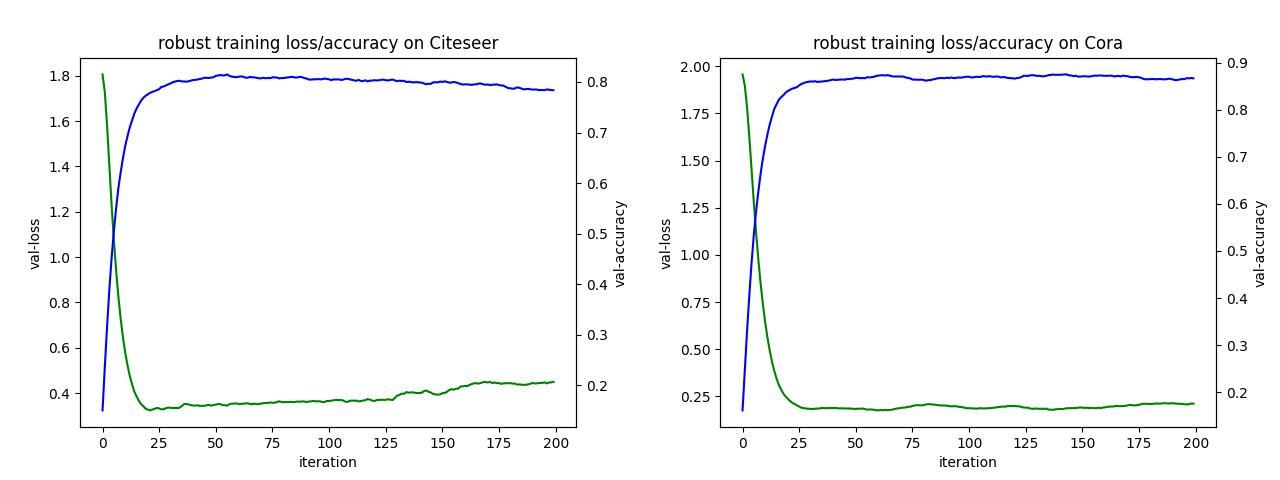
\includegraphics[width=.5\textwidth]{loss-accuracy.jpg} %1.png是图片文件的相对路径
  \caption{the GCN-ICP model validation loss and accuracy curve} %caption是图片的标题
  \label{loss-accuracy} %此处的label相当于一个图片的专属标志,目的是方便上下文的引用
\end{figure}
\subsection{Robust Training Analysis}

Figure \ref{loss-accuracy} illustrates the robust training process of the GCN-ICP model.The left side of the figure presents the validation loss and accuracy curve for the Citeseer dataset, while the right side depicts the same metrics for the Cora dataset, both of them undergo exponential smoothing with a weight of 0.8. Our observations reveal a distinct pattern in the training dynamics:

(i) Rapid Decrease in Validation Loss: As the training progresses, particularly up to around 30 epochs, there is a notable rapid decrease in the validation loss for our GCN-ICP model.
(ii) Stabilization of Metrics: Beyond the initial 30 epochs, both the loss and accuracy metrics tend to stabilize, maintaining a consistent level throughout the remaining iterations.
(iii) Slightly increase in Validation Accuracy: Corresponding to the decrease in validation loss, there is a significant increase in validation accuracy as the model approaches the 30-epoch mark. This increase then plateaus, indicating a stable and effective learning process.


% Figure \ref{loss-accuracy} presents the robust training of the GCN-ICP model. On the left side of the figure, the validation loss and accuracy curve for the Citeseer dataset is displayed, while the right side illustrates the same for the Cora dataset. Through our observations, we note that as the iterations increase to approximately 30 epochs, the validation loss of our GCN-ICP model decreases rapidly. With continued iterations, the loss and accuracy scores stabilize at a consistent level. In terms of validation accuracy, it displays a rapid increase as the iterations approach approximately 30 epochs, and as the iterations continue, it reaches relatively stable scores. The loss and accuracy curves both indicate our model's attainment of both effectiveness and efficiency.

% Table generated by Excel2LaTeX from sheet 'Sheet2'
\begin{table*}[htbp]
  \centering
  \caption{classification accuracy (\%) for the targeted nodes under "PGD" and "Random" attack. Each number is the multi-classification accuracy  after poisoning or evasion attack.}
    \begin{tabular}{|c|c|r|rr|rr|}
    \hline
    \multirow{data} & \multirow{model} & \multicolumn{1}{c|}{\multirow{clean}} & \multicolumn{2}{c|}{evasion attack} & \multicolumn{2}{c|}{poisoning attack} \\
          &       &       & \multicolumn{1}{c}{random} & \multicolumn{1}{c|}{PGD} & \multicolumn{1}{c}{random} & \multicolumn{1}{c|}{PGD} \\
    \hline
    \hline
    \multirow{Cora} & GCN   & 0.823  & 0.788  & 0.748  & 0.737  & 0.735 \\
          & GCNSVD & 0.817  & 0.757  & 0.756  & 0.734  & 0.769  \\
          & GCN-LFR & 0.810  & 0.749  & 0.776  & 0.727  & 0.758  \\
          & GCN-ICP & \textbf{ 0.830 } &\textbf{ 0.804 } & \textbf{ 0.796 } & \textbf{ 0.799 } & \textbf{ 0.781}  \\
    \hline
    \hline
    \multirow{Pubmed} & GCN   & 0.820  & 0.771  & 0.685  & 0.760  & 0.687  \\
          & GCNSVD & 0.817  & \textbf{0.814}  & 0.716  & \textbf{0.811}  & 0.699  \\
          & GCN-LFR & \textbf{0.846}  & 0.694  & \textbf{0.772}  & 0.675  & 0.704  \\
          & GCN-ICP & 0.828  & 0.785  & 0.758  & \textbf{0.770}  & \textbf{0.723}  \\
    \hline
    \hline
    \multirow{Citeseer} & GCN   & 0.712  & 0.656  & 0.659  & 0.647  & 0.649  \\
          & GCNSVD & \textbf{0.718}  & \textbf{0.680}  & 0.672  & 0.644  & 0.671  \\
          & GCN-LFR & 0.688  & 0.412  & 0.587  & 0.406  & 0.572  \\
          & GCN-ICP & 0.698  & 0.672  & \textbf{0.696}  & \textbf{0.657}  & \textbf{0.685}  \\
    \hline
    \end{tabular}%
  \label{tab:non-target-attack}%
\end{table*}%

\section{Conclusion And Feature Works}

In this paper, the GNN-ICP framework is introduced to enhance the learning of diverse representations that effectively capture the graph structure information required for node classification tasks. To increase GNNs robustness, graph features are reconstructed, mutual information is used, and information competition is leveraged to obtain a comprehensive graph representation that defends against target and non-target attacks. 
The robustness of GNN-ICP has been demonstrated by extending it to include GCN-ICP, GAT-ICP and SAGE-ICP models with evasion and poisoning attack experiments. 

Currently, we only consider graph structure perturbations and node classification tasks. Given that graph perturbations occurs on graph structure and node features, down-streaming graph tasks includes link prediction, graph classification and many other unsupervised graph learning. Future work should concentrate on three fields: (i) perturbing graph structure and node feature information while exploring other graph tasks such as link prediction or graph classification. (ii) exploring  many other field datasets and possible experiments, like ZINC\cite{Sterling2015ZINC1} FB15k \cite{Bordes2013TranslatingEF} datasets and knowlege graph models like OAG\cite{Zhang2019OAGTL}. (iii) using different kind of autoregressive graph methods like NetGAN\cite{Bojchevski2018NetGANGG} or GraphAF\cite{Shi2020GraphAFAF} to reconstruct graph structure and node features.

\bibliographystyle{IEEEtran}
\bibliography{IEEEabrv,main}

\end{document}
